\documentclass[11pt]{article}

\usepackage[letterpaper,margin=0.75in]{geometry}
\usepackage{booktabs}
\usepackage{graphicx}
\usepackage{listings}

\setlength{\parindent}{1.4em}

\begin{document}

\lstset{
  language=Python,
  basicstyle=\small,          % print whole listing small
  keywordstyle=\bfseries,
  identifierstyle=,           % nothing happens
  commentstyle=,              % white comments
  stringstyle=\ttfamily,      % typewriter type for strings
  showstringspaces=false,     % no special string spaces
  numbers=left,
  numberstyle=\tiny,
  numbersep=5pt,
  frame=tb,
}

\title{Lab 1 Report}

\author{Jonathan George}

\date{}

\maketitle

\section{Two Nodes - Part 1}



\begin{lstlisting}
class DelayHandler(object):

    def receive_packet(self,packet):
        print Sim.scheduler.current_time(),"\t",packet.ident,"\t",packet.created,"\t",\
            Sim.scheduler.current_time() - packet.created,packet.transmission_delay,"\t",\
            packet.propagation_delay,"\t",packet.queueing_delay

_1MBPS = 1000000
_1GBPS = _1MBPS * 1000

def run():
    print "time\t","ident\t","created\t", "sent_at\t", "Dtrans\t", "Dprop\t", "Dqueue\t"
    Sim.scheduler.run()

def twoNodeSetUp():
    # parameters
    Sim.scheduler.reset()

    # setup network
    net = Network('twoNodes.txt')

    # setup routes
    n1 = net.get_node('n1')
    n2 = net.get_node('n2')
    n1.add_forwarding_entry(address=n2.get_address('n1'),link=n1.links[0])
    n2.add_forwarding_entry(address=n1.get_address('n2'),link=n2.links[0])

    # setup app
    d = DelayHandler()
    net.nodes['n2'].add_protocol(protocol="delay",handler=d)
    return n1,n2

"""
Set the bandwidth of the links to 1 Mbps, with a propagation delay of 1 second. 
Send one packet with 1000 bytes from n1 to n2 at time 0.
"""
def twoNodes_1():
    n1,n2 = twoNodeSetUp()

    n1.links[0].bandwidth = _1MBPS
    n2.links[0].bandwidth = _1MBPS
    n1.links[0].propagation = 1;
    n2.links[0].propagation = 1;

    # send one packet
    p = packet.Packet(destination_address=n2.get_address('n1'),
                        ident=1,protocol='delay',length=1000)
    Sim.scheduler.add(delay=0, event=p, handler=n1.send_packet)
    # run the simulation
    run()
\end{lstlisting}

Output
1MBPS bandwidth - Dprop 1 sec - one 1000 byte packet
time    ident   created sent_at Dtrans  Dprop   Dqueue  
1.008   1       0       1.008   0.008   1       0

\section{Two Nodes - Part 2}

Lorem ipsum dolor sit amet, consectetur adipiscing elit. Suspendisse
posuere tellus scelerisque ante luctus eget dapibus ante
egestas. Pellentesque habitant morbi tristique senectus et netus et
malesuada fames ac turpis egestas. Curabitur eget lacus massa, eget
venenatis nisi. Mauris auctor posuere dignissim. Aenean nec tortor
ante, in venenatis arcu. Sed velit turpis, hendrerit ut feugiat
viverra, ultricies tempus nulla. Pellentesque molestie leo ac mi
aliquet sit amet faucibus enim interdum. Phasellus quis sapien
odio. Suspendisse tempor malesuada quam, eget elementum elit placerat
nec. Ut id laoreet risus.

\begin{lstlisting}
"""
Set the bandwidth of the links to 100 bps, with a propagation delay of 10 ms. 
Send one packet witih 1000 bytes from n1 to n2 at time 0.
"""
def twoNodes_2():
    n1,n2 = twoNodeSetUp()

    n1.links[0].bandwidth = 100
    n2.links[0].bandwidth = 100
    n1.links[0].propagation = 0.010 #10 ms
    n2.links[0].propagation = 0.010 #10 ms

    # send one packet
    p = packet.Packet(destination_address=n2.get_address('n1'),
                        ident=1,protocol='delay',length=1000)
    Sim.scheduler.add(delay=0, event=p, handler=n1.send_packet)

    run()


\end{lstlisting}
Output:
100bps bandwidth - Dprop 10 ms - one 1000 byte packet
time    ident   created sent_at Dtrans  Dprop   Dqueue  
80.01   1       0       80.01   80.0    0.01    0

\section{Two Nodes - Part 3}

Lorem ipsum dolor sit amet, consectetur adipiscing elit. Suspendisse
posuere tellus scelerisque ante luctus eget dapibus ante
egestas. Pellentesque habitant morbi tristique senectus et netus et
malesuada fames ac turpis egestas. Curabitur eget lacus massa, eget
venenatis nisi. Mauris auctor posuere dignissim. Aenean nec tortor
ante, in venenatis arcu. Sed velit turpis, hendrerit ut feugiat
viverra, ultricies tempus nulla. Pellentesque molestie leo ac mi
aliquet sit amet faucibus enim interdum. Phasellus quis sapien
odio. Suspendisse tempor malesuada quam, eget elementum elit placerat
nec. Ut id laoreet risus.

\begin{lstlisting}
"""
Set the bandwidth of the links to 1 Mbps, with a propagation delay of 10 ms. 
Send three packets from n1 to n2 at time 0 seconds, then one packet at time 2 seconds. 
All packets should have 1000 bytes.
"""
def twoNodes_3():
    n1,n2 = twoNodeSetUp()

    n1.links[0].bandwidth = _1MBPS
    n2.links[0].bandwidth = _1MBPS
    n1.links[0].propagation = 0.010 #10 ms
    n2.links[0].propagation = 0.010 #10 ms

    # send three packet
    p = packet.Packet(destination_address=n2.get_address('n1'),
                        ident=1,protocol='delay',length=1000)
    Sim.scheduler.add(delay=0, event=p, handler=n1.send_packet)
    p = packet.Packet(destination_address=n2.get_address('n1'),
                        ident=1,protocol='delay',length=1000)
    Sim.scheduler.add(delay=0, event=p, handler=n1.send_packet)
    p = packet.Packet(destination_address=n2.get_address('n1'),
                        ident=1,protocol='delay',length=1000)
    Sim.scheduler.add(delay=0, event=p, handler=n1.send_packet)

    #One more at t=2
    p = packet.Packet(destination_address=n2.get_address('n1'),
                        ident=1,protocol='delay',length=1000)
    Sim.scheduler.add(delay=2, event=p, handler=n1.send_packet)

    run()
\end{lstlisting}
Output:
1Mbps bandwidth - Dprop 10 ms - three 1000 byte packet, one more at t=2
time    ident   created sent_at Dtrans  Dprop   Dqueue  
0.018   1       0       0.018   0.008   0.01    0
0.026   1       0       0.026   0.008   0.01    0.008
0.034   1       0       0.034   0.008   0.01    0.016
2.018   1       2.0     0.018   0.008   0.01    0.0


\section{Three Nodes - Two Fast Links}

Description of the two fast links setup. 

\begin{lstlisting}
def threeNodeSetup():
    # parameters
    Sim.scheduler.reset()

    # setup network
    net = Network('threeNodes.txt')

    # setup routes
    n1 = net.get_node('n1')
    n2 = net.get_node('n2')
    n3 = net.get_node('n3')
    n1.add_forwarding_entry(address=n2.get_address('n1'),link=n1.links[0])
    n1.add_forwarding_entry(address=n3.get_address('n2'),link=n1.links[0])
    n2.add_forwarding_entry(address=n1.get_address('n2'),link=n2.links[0])
    n2.add_forwarding_entry(address=n3.get_address('n2'),link=n2.links[1])
    n3.add_forwarding_entry(address=n1.get_address('n2'),link=n3.links[0])
    n3.add_forwarding_entry(address=n2.get_address('n3'),link=n3.links[0])

    # setup app
    d = DelayHandler3Node()
    net.nodes['n3'].add_protocol(protocol="delay",handler=d)
    
    return n1,n2,n3

#def sendPacket(src, dest):


"""
Two fast links - 1MBPS - 100ms

Node A transmits a stream of 1 kB packets to node C. 
How long does it take to transfer a 1 MB file, divided into 1 kB packets, from A to C? 
Which type of delay dominates?
"""
def fastLinks():
    n1,n2,n3 = threeNodeSetup()

    n1.links[0].bandwidth = _1MBPS
    n2.links[0].bandwidth = _1MBPS
    n2.links[1].bandwidth = _1MBPS
    n3.links[0].bandwidth = _1MBPS

    n1.links[0].propagation = 0.100 #100 ms
    n2.links[0].propagation = 0.100 #100 ms
    n2.links[1].propagation = 0.100 #100 ms
    n3.links[0].propagation = 0.100 #100 ms



    for i in range(0,1000):
        p = packet.Packet(destination_address=n3.links[0].address,
                        ident=i,protocol='delay',length=1000)
        Sim.scheduler.add(delay=0, event=p, handler=n1.send_packet)

    Sim.scheduler.run()

"""
If both links are upgraded to a rate of 1 Gbps, 
how long does it take to transfer a 1 MB file from A to C?
"""
def fasterLinks():
    n1,n2,n3 = threeNodeSetup()

    n1.links[0].bandwidth = _1GBPS
    n2.links[0].bandwidth = _1GBPS
    n2.links[1].bandwidth = _1GBPS
    n3.links[0].bandwidth = _1GBPS

    n1.links[0].propagation = 0.100 #100 ms
    n2.links[0].propagation = 0.100 #100 ms
    n2.links[1].propagation = 0.100 #100 ms
    n3.links[0].propagation = 0.100 #100 ms

    for i in range(0,1000):
        p = packet.Packet(destination_address=n3.links[0].address,
                        ident=i,protocol='delay',length=1000)
        Sim.scheduler.add(delay=0, event=p, handler=n1.send_packet)

    Sim.scheduler.run()
\end{lstlisting}
Fast Links
End Time: 8.208
Queueing delay: 7.992

Faster Links
End Time: 0.208008
Queueing delay: 0.007992

Anaysis of the results

\section{Three Nodes - One Slow link}

Lorem ipsum dolor sit amet, consectetur adipiscing elit. Suspendisse
posuere tellus scelerisque ante luctus eget dapibus ante
egestas. Pellentesque habitant morbi tristique senectus et netus et
malesuada fames ac turpis egestas. Curabitur eget lacus massa, eget
venenatis nisi. Mauris auctor posuere dignissim. Aenean nec tortor
ante, in venenatis arcu. Sed velit turpis, hendrerit ut feugiat
viverra, ultricies tempus nulla. Pellentesque molestie leo ac mi
aliquet sit amet faucibus enim interdum. Phasellus quis sapien
odio. Suspendisse tempor malesuada quam, eget elementum elit placerat
nec. Ut id laoreet risus.

\begin{lstlisting}
"""
One fast link and one slow link - 1MBPS/256KBPS - 100ms

Node A transmits 1000 packets, each of size 1 kB, to node C. 
How long would it does it take to transfer a 1 MB file, divided into 1 kB packets, from A to C?
"""
def slowLink():
    n1,n2,n3 = threeNodeSetup()

    n1.links[0].bandwidth = _1MBPS
    n2.links[0].bandwidth = _1MBPS
    n2.links[1].bandwidth = 256*1000 #256Kbps
    n3.links[0].bandwidth = 256*1000 #256Kbps

    n1.links[0].propagation = 0.100 #100 ms
    n2.links[0].propagation = 0.100 #100 ms
    n2.links[1].propagation = 0.100 #100 ms
    n3.links[0].propagation = 0.100 #100 ms

    for i in range(0,1000):
        p = packet.Packet(destination_address=n3.links[0].address,
                        ident=i,protocol='delay',length=1000)
        Sim.scheduler.add(delay=0, event=p, handler=n1.send_packet)
    Sim.scheduler.run()
\end{lstlisting}
Fast/Slow Links
End Time: 31.458
Queueing delay: 31.21875

\section{Queueing Theory}

Donec luctus, libero et egestas tincidunt, arcu ante commodo nunc,
quis sodales leo risus non libero. Mauris ac blandit ligula. Praesent
in dolor non nibh congue blandit. Curabitur in sodales
neque. Curabitur tincidunt nisl nec mauris bibendum
molestie. Suspendisse non justo erat. Ut quis odio elit, sit amet
ullamcorper dui. Nam massa urna, tempus non hendrerit porttitor,
feugiat quis quam. Quisque lacinia cursus nulla, id placerat enim
accumsan et. Donec porta pharetra tincidunt.

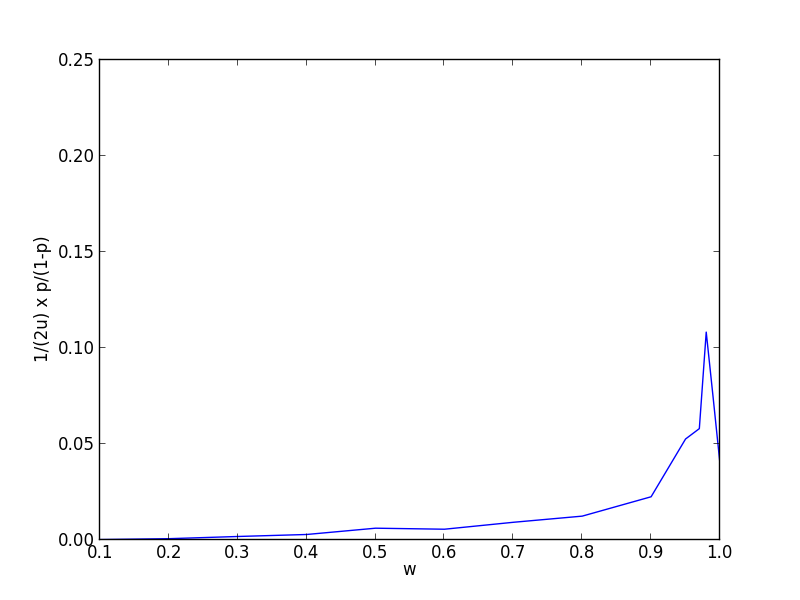
\includegraphics[width=11cm]{equation.png}

\end{document}